% LAB 6: File I/O
% 
% CSE/IT 107: Introduction to Programming
% New Mexico Tech
% 
% Prepared by Russell White and Christopher Koch
% Spring 2015
\documentclass[11pt]{cselabheader}

%%%%%%%%%%%%%%%%%% SET TITLES %%%%%%%%%%%%%%%%%%%%%%%%%
\fancyhead[R]{Lab 6: File I/O}
\title{Lab 6: File I/O}

\begin{document}

\maketitle

\hrule
\begin{quotation}
``The danger that computers will become like humans is not as big as the danger
that humans will become like computers.'' (``Die Gefahr, dass der Computer so
wird wie der Mensch ist nicht so gro\ss, wie die Gefahr, dass der Mensch so wird
wie der Computer.'')
\end{quotation}
\begin{flushright}
--- Konrad Zuse
\end{flushright}

\begin{quotation}
	``First, solve the problem. Then, write the code.''
\end{quotation}
\begin{flushright}
	--- John Johnson
\end{flushright}

\begin{quotation}
``I don’t need to waste my time with a computer just because I am a computer
scientist.''
\end{quotation}
\begin{flushright}
--- Edsger W. Dijkstra
\end{flushright}

\hrule

\section{Introduction}
In previous labs, we taught you how to use functions, math, lists, strings, and
the like. We will combine all that in this lab and teach you how to interact
with files. This will lead us to do some exciting data analysis!

\section{I/O Exceptions}
When working with input and output it is important to check for exceptions.  For example, when we try to open a file that does not exist we'd like to exit the program safely or recover rather than observing the unexpected results.  Exception handling in python consists of "try-except" blocks.  In a "try-except" block we execute instructions in the \pythoninline!try! block and catch errors in one or more following \pythoninline!except! blocks.  The \pythoninline!except! block is only executed if an exception is caught in the \pythoninline!try! block.  Additionally, when an error is caught in the \pythoninline!try! block we stop executing commands in the \pythoninline!try! block and jump to the first \pythoninline!except! or optional \pythoninline!finally! block.  The following example throws a division by zero error and prints ``division by zero'':

\begin{python3code}
prime = 7
x = 0

try:
  result = prime / 0
  result = 7*42

except ZeroDivisionError as err:
  print(err)
\end{python3code}

Looking at the code above, since the error is thrown on line 5, line 4 is never executed.  Any \pythoninline!except!  block that does not list built-in  exceptions will catch all exceptions not listed in previous \pythoninline!except! blocks.  For example, the following code will throw an error if the user enters anything but an integer:

\begin{python3code}
try:
  x = int(input("Enter a number: "))

except:
  print("Unknown error.")
  raise
else:
  print("You entered: " + str(x))
\end{python3code}

The \pythoninline!raise! keyword causes a stack trace and prints out additional information if an exception is encountered.  The \pythoninline!else! block is always optional and will always be executed if no exceptions are thrown in the \pythoninline!try! block.  There are many more built-in exceptions such as \pythoninline!IOError! that can be found here: \url{https://docs.python.org/3.2/library/exceptions.html}

If you try to open a file that does not exist for reading, Python will display
an error message:

\begin{pyconcode}
>>> open("not_a_file.txt", "r")
Traceback (most recent call last):
  File "<pyshell#0>", line 1, in <module>
  open("not_a_file.txt", "r")
FileNotFoundError: [Errno 2] No such file or directory: 'not_a_file.txt'
\end{pyconcode}

In this case, the error is \pythoninline!IOError!. Normally having an
error occur will end your program, but we can use \pythoninline!try-except! in
order to perform a special action in case of an error. The following program
uses this to display an error message rather than crashing.

\begin{python3code}
filename = input("What file should be read? ")

try:
  input_file = open(filename, "r")
  for line in input_file:
    print(line, end="")

except IOError as err:
  print(err)
  raise
else:
  input_file.close()
finally:
  print("Goodbye!")
\end{python3code}

Lastly, the \pythoninline!finally! block is where clean-up actions are performed and is always executed after leaving the \pythoninline!try! block.
\section{File I/O}
Knowing how to work with files is important, since it lets us store and retrieve
data beyond the scope of the single execution of a program. To open a file for
reading or writing we will use the \pythoninline!open! function. The following
example opens a file and writes ``Hello World'' to it.

\begin{python3code}
output_file = open("hello.txt", "w")

print("Hello World", file=output_file)
output_file.close()
\end{python3code}

Files can also be written to by using \pythoninline!.write(contents)!. This method will write only the characters given to it, so a newline \lstinline{\\n} must be included for a newline.

\begin{python3code}
output_file = open("hello.txt", "w")

output_file.write("Hello World\n")
output_file.close()
\end{python3code}

The arguments to the \pythoninline!open! function are, in order, the name of the
file to open and the mode in which to open the file. ``w'' means that the file
is to be opened in write mode. If the file does not exist, this will create the
file. If it does exist, then the contents of the file will be cleared in
preparation for the new ones.

Other options include ``a'', which is similar to ``w'' but will not clear the
contents of an existing file and will instead append the new data to the end,
and ``r'' which will read the file instead. If ``r'' is used and the file does
not exist, then an error will occur. The following code takes a filename as user
input, then prints out the entire contents of that file.

\begin{table}[!ht]
  \centering
  \begin{tabular}{ll}
    Mode & What it does \\
    \midrule
    a & Create file if does not exist, open file, append contents to the end \\
    w & Create file if does not exist, open file, write contents to the beginning
    of file \\
    r & Open file, permit reading only \\
  \end{tabular}
\end{table}

\begin{python3code}
filename = input("What file should be read? ")

input_file = open(filename, "r")
for line in input_file:
  print(line, end="")

input_file.close()
\end{python3code}

The additional concepts introduced in these examples are:

\begin{itemize}
\item The \pythoninline!print! function can have an additional ``file'' parameter
  passed to it to allow writing to a file. This causes it to send its output to
  the file rather than the screen, though otherwise it performs identically.

\item The \pythoninline!print! function has an additional optional ``end''
  parameter. This allows you to specify what should be printed after the main
  string given to it. This is important because it defaults to \pythoninline!"\n"!,
  which causes a newline after every print statement. By changing ``end'' to
  \pythoninline!""! we prevent a newline from being added after every line of the
  file is printed. This is because each line in the file already has a newline
  at the end of it, so we don't need \pythoninline!print! to add its own.

\item \pythoninline!.close()! is used to properly tell Python that you are done
  with a file and close your connection to it. This isn't \emph{strictly}
  required, but without it you risk the file being corrupted or other programs
  being unable to access that file.

\item When reading from a file, Python can use a \pythoninline!for! loop to go
  through each line in sequence. This works identically to if you think of the
  file as a list with every line being a different element of the list. The
  entirety of the file can also be read into a single string using the
  \pythoninline!.read()! function.

\begin{pyconcode}
>>> input_file = open("test.py", "r")
>>> contents = input_file.read()
>>> print(contents)
filename = input("What file should be read? ")

input_file = open(filename, "r")
for line in input_file:
  print(line, end="")

input_file.close()
\end{pyconcode}

\item \pythoninline!.readlines()! can be used to read all of a file at once, though
  it splits the file into a list. Each element of the list will be one line of
  the file being read.
\end{itemize}

\subsection{Files Using \pythoninline!with!}
Since every file that you open should be closed after use, Python has an easy way to do this for you. Using the \pythoninline!with! command, your file will automatically be closed when the \pythoninline!with! block finished executing.

\begin{python3code}
filename = input("Enter filename: ")

with open(filename, "r") as file:
  for line in file:
    print(line, end="")
# file.close() is not necessary, because ``with'' closed it for us
\end{python3code}


\subsection{Error Handling}
If you try to open a file that does not exist for reading, Python will display
an error message:

\begin{pyconcode}
>>> open("not_a_file.txt", "r")
Traceback (most recent call last):
  File "<pyshell#0>", line 1, in <module>
  open("not_a_file.txt", "r")
FileNotFoundError: [Errno 2] No such file or directory: 'not_a_file.txt'
\end{pyconcode}

In this case, the error is \pythoninline!FileNotFoundError!. Normally having an
error occur will end your program, but we can use \pythoninline!try-except! in
order to perform a special action in case of an error. The following program
uses this to display an error message rather than crashing.

\begin{python3code}
filename = input("What file should be read? ")

try:
  input_file = open(filename, "r")
  for line in input_file:
    print(line, end="")

  input_file.close()
except FileNotFoundError:
  print("Could not find file {}.".format(filename))
\end{python3code}

If you wish to catch an error, check the error message for the name of the error
that you need to catch with your \pythoninline!except! statement. If the specified
error does not occur inside the \pythoninline!try! block, then the
\pythoninline!except! block will be skipped. A single \pythoninline!try! block can
have several \pythoninline!except! statements following it for catching multiple
types of errors.

%\section{Recursion}
\pagebreak
\section{Instantiating Turtles}
Similarly to being able to open multiple files, we can also create multiple
turtles to draw more complex designs. This is done using the
\pythoninline!turtle.Turtle()! function. This function returns a turtle object,
which we can call every other normal turtle function on.

\begin{python3code}
import turtle

first = turtle.Turtle()
second = turtle.Turtle()

first.forward(50)
second.forward(50)
first.left(90)
second.right(90)
first.forward(50)
second.forward(50)
first.right(90)
second.left(90)
first.forward(50)
second.forward(50)
\end{python3code}

\begin{figure}[h]
  \centering
  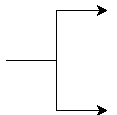
\includegraphics[width=1.0in]{img/turtle_prong}
\end{figure}

If we add a group of turtles to a list, we can easily apply the same commands to all of them, as in this example:

\begin{python3code}
import turtle

turtles = []
first = turtle.Turtle()
first.speed(0)
turtles.append(first)

second = turtle.Turtle()
second.speed(0)
second.right(90)
turtles.append(second)

third = turtle.Turtle()
third.speed(0)
third.right(180)
turtles.append(third)

fourth = turtle.Turtle()
fourth.speed(0)
fourth.right(270)
turtles.append(fourth)

for i in range(200):
    for turt in turtles:
        turt.forward(i/5)
        turt.left(10)
\end{python3code}

\begin{figure}[h]
  \centering
  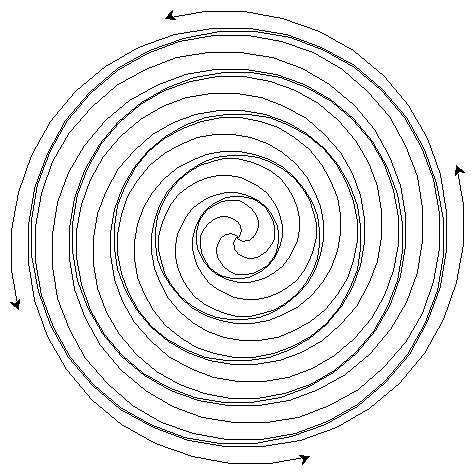
\includegraphics[width=2.0in]{img/fancy_spiral}
\end{figure}

\section{Matplotlib}
Matplotlib is a Python library that provides MATLAB-like plotting functions.  Simple plots such as bar graphs and line graphs are very easy to create using matplotlib.\\
Using the \pythoninline!.plot! and \pythoninline!.bar! methods of \pythoninline!matplotlib.pyplot!, we can quickly show line and bar graphs. \pythoninline!.plot! and \pythoninline!.bar! take a dataset for x and a dataset for y, with many more optional parameters such as \pythoninline!align!.  These examples use data from \url{nmt.edu/~olegm/382labs/2cities.csv}.

\begin{python3code}
import matplotlib.pyplot as plt

with open("2cities.csv", "r") as f:
        lines = f.readlines()

t = []
for l in lines:
        a = l.split()
        if len(a) > 1:
                t.append(a[1])
t.pop(0)
ts = []
for i in t:
        ts.append(float(i))

x = list(range(1,11))

y = []
for i in x:
        y.append([])
        for j in ts:
                if j > (i - 1) * 5 and j < i * 5:
                        y[i - 1].append(j)

yc = []
for i in y:
        yc.append(len(i))

plt.bar(x, yc, align="center")
plt.xlabel("X-Axis")
plt.ylabel("Y-Axis")
plt.title("Title")
plt.show()
\end{python3code}

This code will produce this output of the input data sorted into 10 bins of size 5 (not showing empty bins):\\
\begin{figure}[h]
  \centering
  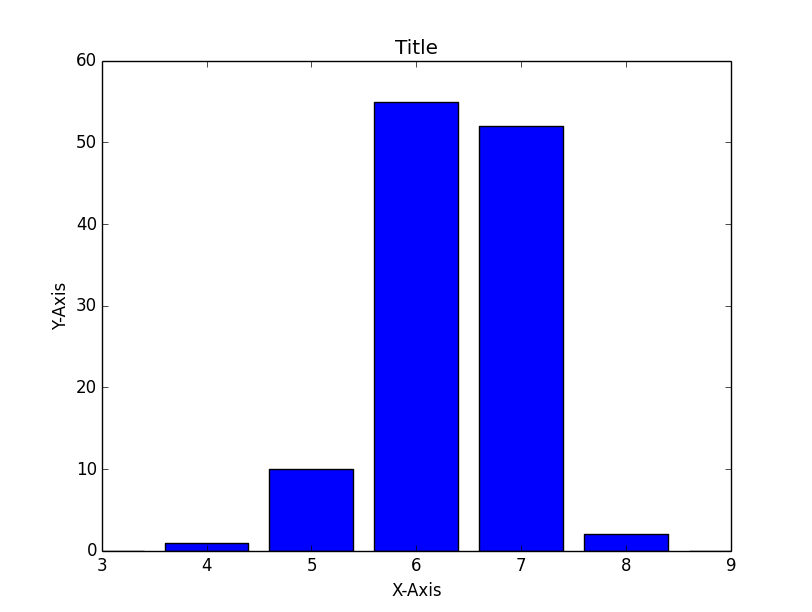
\includegraphics[width=4.0in]{img/bar1}
\end{figure}

Likewise, the following code will show a line plot of the dataset:\\
\begin{python3code}
import matplotlib.pyplot as plt

with open("2cities.csv", "r") as f:
        lines = f.readlines()

t = []
for l in lines:
        a = l.split()
        if len(a) > 1:
                t.append(a[1])
t.pop(0)
ts = []
for i in t:
        ts.append(float(i))

x = list(range(len(ts)))

plt.plot(x, ts)
plt.xlabel("X-Axis")
plt.ylabel("Y-Axis")
plt.title("Title")
plt.show()
\end{python3code}

\begin{figure}[h]
  \centering
  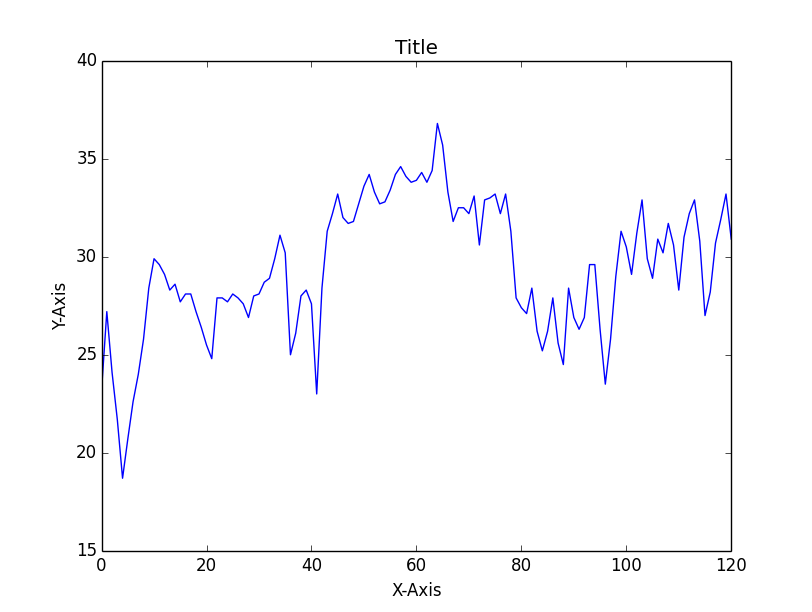
\includegraphics[width=4.0in]{img/line1}
\end{figure}

\pagebreak
\section{Exercises}
\label{sec:ex}

\begin{ex}[save.py] Write a program that takes in a filename, then takes in
  a series of lines of input until a blank line is entered, writing each line to
  the file with the given name. After the blank line is entered, properly close
  the file before ending the program.  
\end{ex}

\begin{ex}[word\_count.py] Write a program that
  takes in a filename and string as input. Then print how many times that string
  appears inside the chosen file. If the file does not exist, continue asking
  for a filename until one is given that exists. Use your source code file as
  test input.
\end{ex}

\begin{ex}[navigate3.py] Modify navigate.py so that, rather than take instructions
    from the command line, it reads from a file (specified by user input) to
    determine what the turtle will do. Additionally, you will be adding the
    ``split'' command. This command will use instantiation of new turtles in order
    to draw multiple lines at once. Every new command will apply to every turtle
    that currently exists. The file will have on instruction per line. The
    possible instructions are:

    \begin{description}
      \item[forward X] Move all turtles forward X.
      \item[left X] Turn all turtles X degrees to the left.
      \item[right X] Turn all turtles X degrees to the right.
      \item[split X] Split all turtles into new turtles. Each new turtle will be turned X degrees to the right.
    \end{description}

    In order to properly implement split, you will probably need to look up the
turtle functions \pythoninline!.position()!, \pythoninline!.setposition()!,
    \pythoninline!.setheading()!, \pythoninline!.heading()!, \pythoninline!.penup()!, and
    \pythoninline!.pendown()!. Turtle documentation is available at
    \url{https://docs.python.org/3/library/turtle.html}.

    You will also likely use the \pythoninline!.split()! command when getting input, which splits a single string into an array around the string's spaces.
    \begin{pyconcode}
>>> print("this is a phrase".split())
['this', 'is', 'a', 'phrase']
>>> print("hi,hi,hi".split(",")
['hi', 'hi', 'hi']
    \end{pyconcode}

    \emph{Suggestion:} Split each command into a different function to help keep their logic separate.

    Sample Input File:
    \begin{python3code}
forward 50
left 20
split 40
forward 50
left 20
split 40
forward 50
left 20
split 40
forward 50
left 20
split 40
forward 50
left 20
    \end{python3code}

    Sample Output
    \begin{center}
      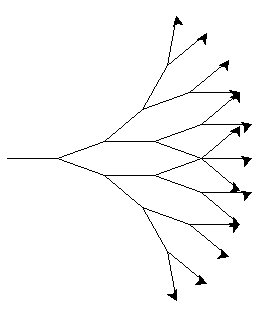
\includegraphics[width=1.0in]{img/nav3_example}
    \end{center}
  \end{ex}

	\begin{ex}[diff.py]
		Write a ``diff'' program that prints out the differences, line by line, of two files.  Your program should ask the user for the names of two files, then print the differences between them.  Follow the format output by the system ``diff'' utility.  Make sure to use proper error handling techniques for file I/O.\\\\
		Example:\\\\
		file1.txt:
		\begin{python3code}
		John goes to work.
		Keith and Kyle went to the Ensiferum concert.
		Alice ate an apple pie.
		Joe cut down a tree.
		The dog jumped over the wall.
		\end{python3code}
		file2.txt:
		\begin{python3code}
		John goes to work.
		Coral went to a Kesha concert.
		Alice ate an apple pie.
		Joe planted a tree.
		The dog jumped over the wall.
		\end{python3code}
		\begin{python3code}
		Enter file name 1: >>> file1.txt
		Enter file name 2: >>> file2.txt
		
		2c2
		< Keith and Kyle went to the Ensiferum concert.
		---
		> Coral went to a Kesha concert.
		4c4
		< Joe cut down a tree.
		---
		> Joe planted a tree.
		\end{python3code}
	\end{ex}


\pagebreak
\section{Submitting}

You should submit your code as a tarball. It should contain all files
used in the exercises for this lab. The submitted file should be named
\begin{center}
  \texttt{cse107\_firstname\_lastname\_lab6.tar.gz}
\end{center}

\begin{center}
  \textbf{Upload your tarball to Canvas.}
\end{center}

\listoftheorems


\end{document}
